

\subsection{Scaling complexity of the task pool}
\label{app:scaling_complexity}

One final axis along which it is possible to scale our method is the overall complexity of the task distribution. We compare our main task distribution, as described in Section \ref{sec:methods_xverse} and Appendix \ref{app:presample_tasks} to a subset which maintains the use of the same goals, production rules, and objects, but eliminates any navigational complexity by having a single world topology: an empty room. Recall that we count the number of tasks as the product of number of worlds and the number of games. To disentangle the effects of scaling complexity versus scaling the sheer number of tasks, we add 5,000 unique object initialisation points for the empty room. These serve as the proxy ``4,000 worlds'' and are, by design, much less diverse and complex than the 4,000 worlds in the main training pool.\footnote{Note that the distribution over world topologies we use here is smaller than the distribution used in the model scaling experiments in Section \ref{sec:scaling_results}, and results are therefore not comparable across these sections.} For more details of the experimental setup, see Appendix \ref{app:task-complexity-scaling} and Table ~\ref{tab:task_complexity_scaling}.

In Figure \ref{fig:task_complexity_scaling}, we show that low environment complexity can be a bottleneck to scaling, by comparing the effectiveness of model scaling between agents trained on the two distributions, and each evaluated on their respective test sets. On both the median (Figure \ref{subfig:complexity-scaling-empty-room-50th}) and 20\textsuperscript{th} (Figure \ref{subfig:complexity-scaling-empty-room-20th}) percentiles in the empty room, we see that past a certain point (42M Transformer parameters), scaling model size begins to reduce performance. By contrast, in the distribution with many world topologies (Figures \ref{subfig:complexity-scaling-worlds-50th} and \ref{subfig:complexity-scaling-worlds-20th}), increased model size continues to improve performance far beyond this, showing improvements through at least 75M Transformer parameters.
Open-ended settings with unbounded environment complexity, such as multi-agent systems, may therefore be particularly important for scaling up adaptive agents.


\begin{figure}[t!]
    \centering
    \begin{subfigure}[b]{0.49\textwidth}
        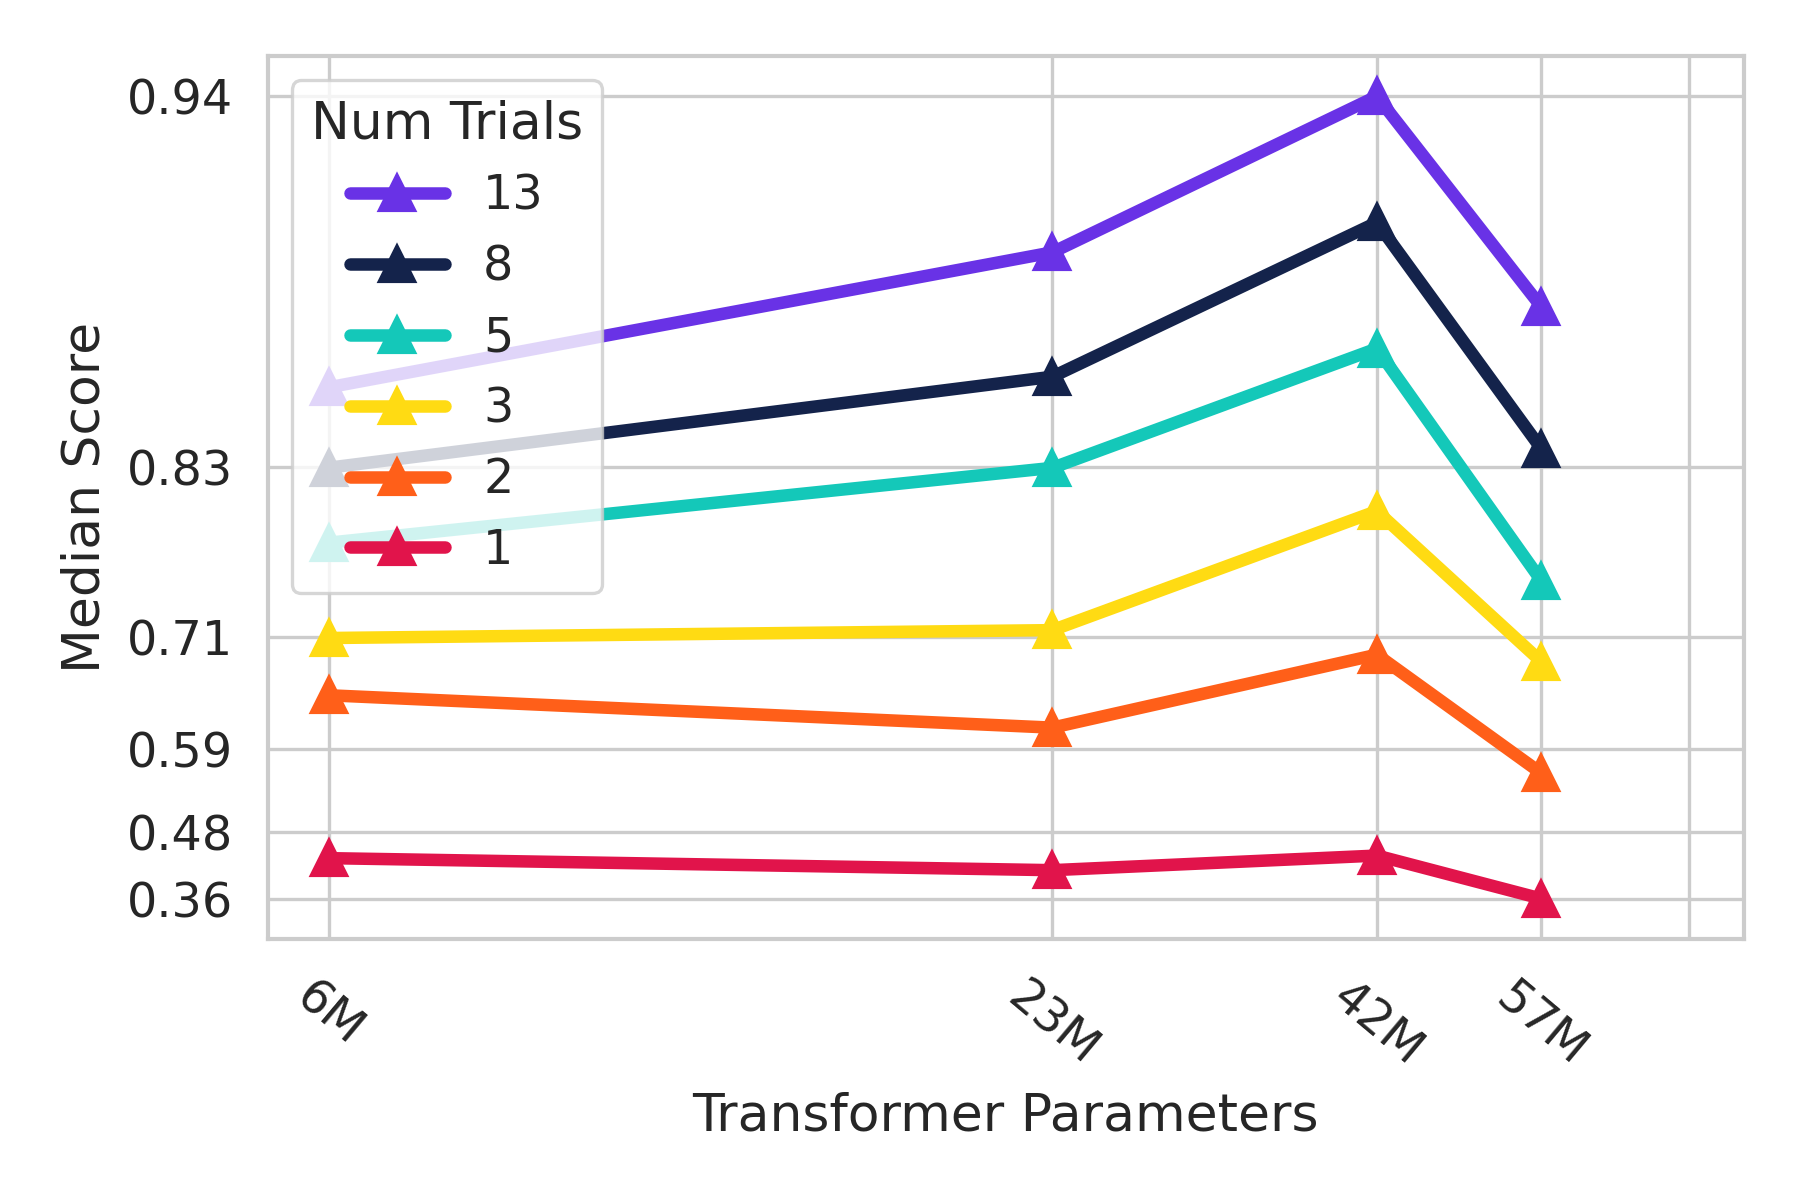
\includegraphics[width=\textwidth]{figures/scaling/emptyroom_parameter_scaling_percentile50.png}
        \caption{\centering Task distribution with only empty room inhibits scaling (median).}
        \label{subfig:complexity-scaling-empty-room-50th}
    \end{subfigure}
    \hfill
    \begin{subfigure}[b]{0.49\textwidth}
        \centering
        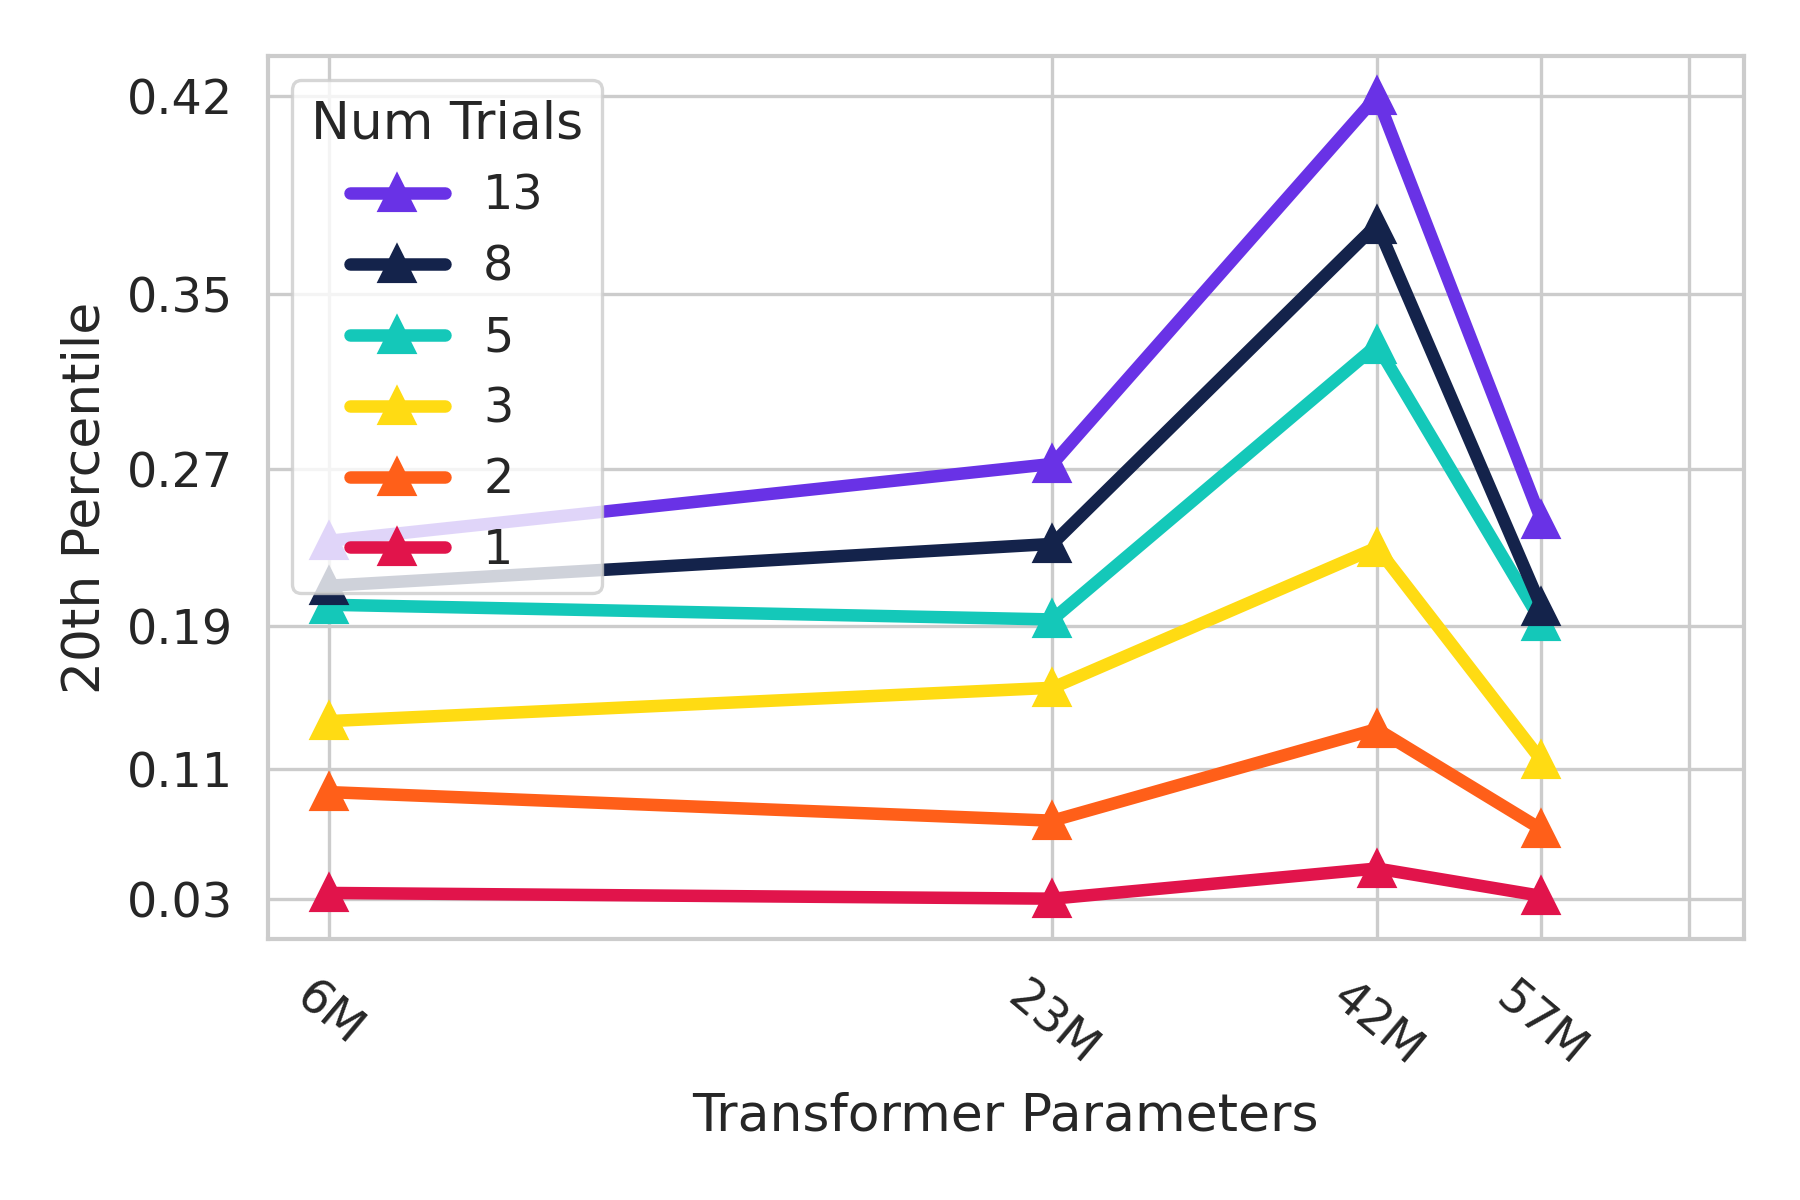
\includegraphics[width=\textwidth]{figures/scaling/emptyroom_parameter_scaling_percentile20.png}
        \caption{\centering Task distribution with only empty room inhibits scaling (20th percentile).}
        \label{subfig:complexity-scaling-empty-room-20th}
    \end{subfigure}
    
    \vspace{2mm}
    
    \begin{subfigure}[b]{0.49\textwidth}
        \centering
        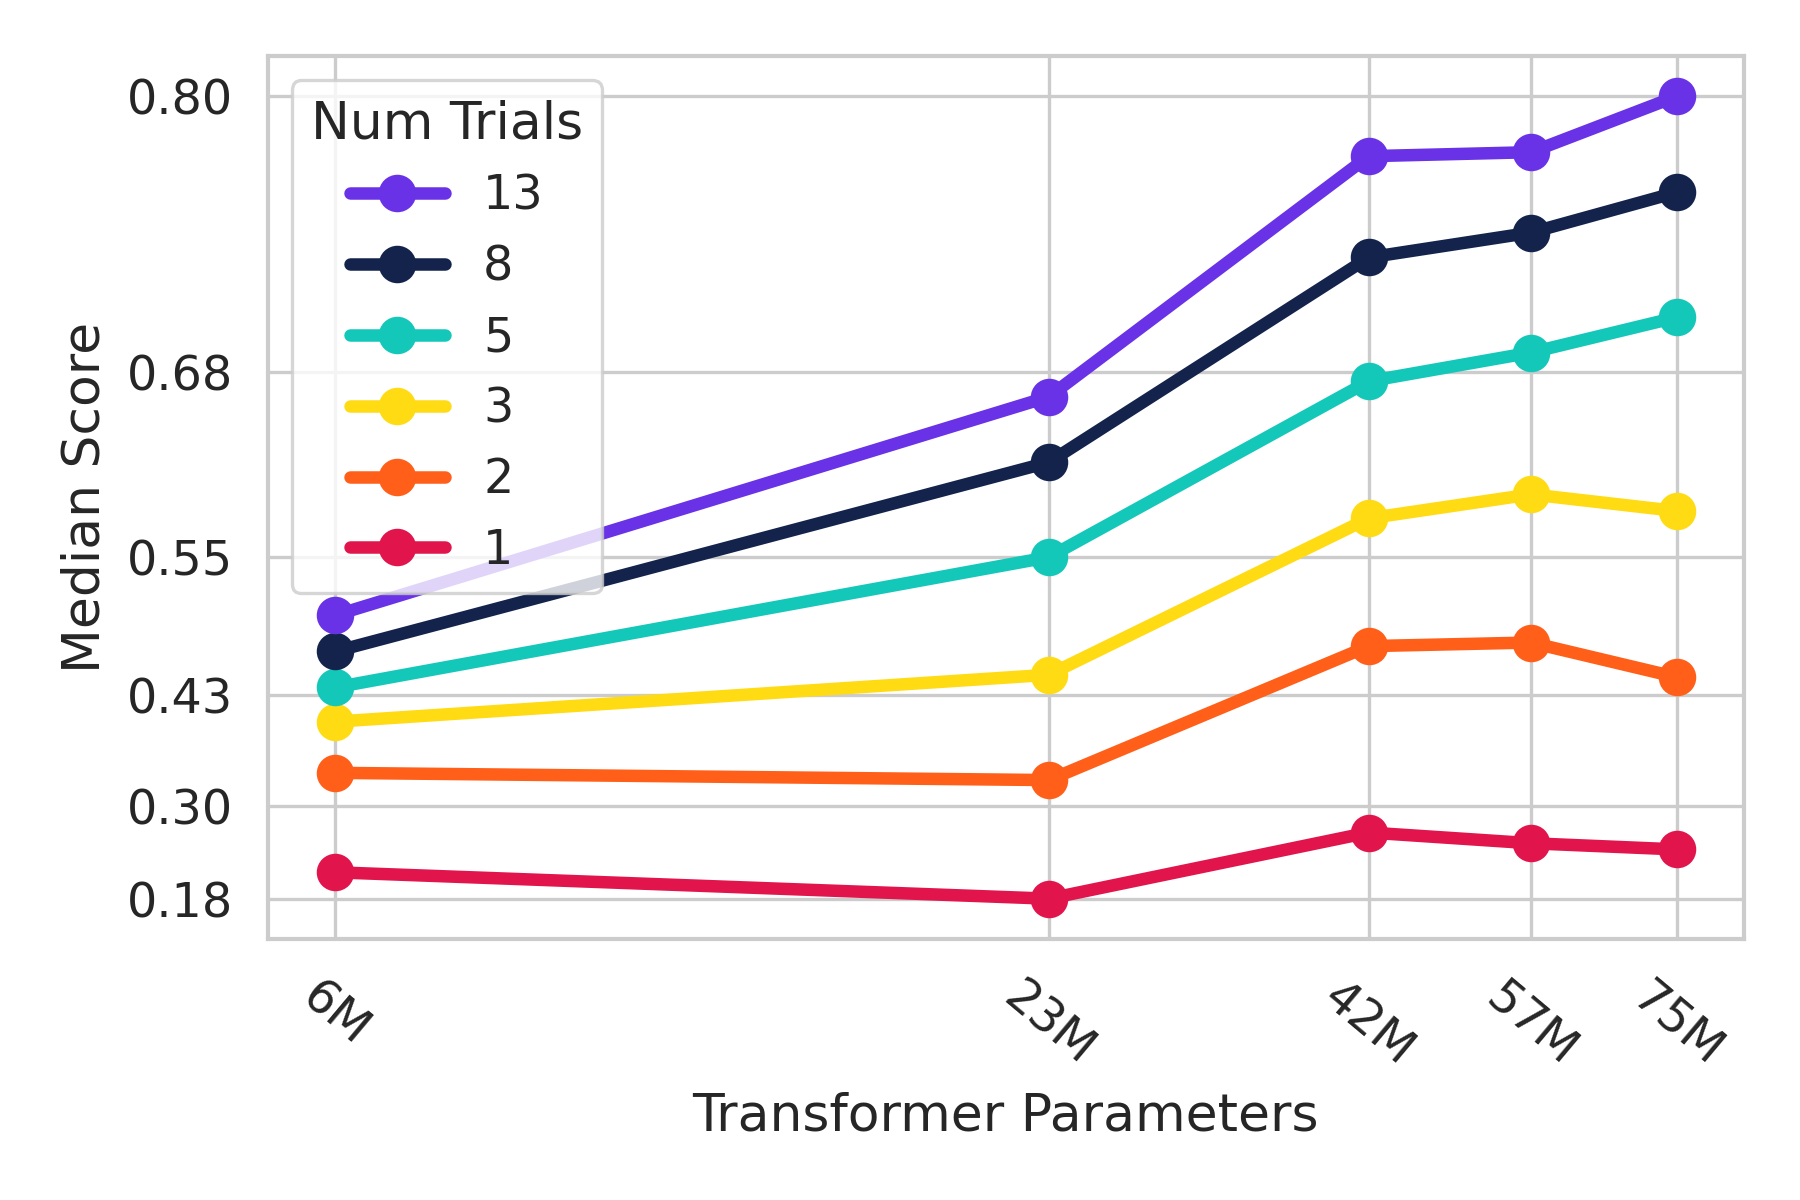
\includegraphics[width=\textwidth]{figures/scaling/worlds_complexity_parameter_scaling_percentile50.png}
        \caption{\centering Task distribution with many world topologies facilitates scaling (median).}
        \label{subfig:complexity-scaling-worlds-50th}
    \end{subfigure}
    \hfill
    \begin{subfigure}[b]{0.49\textwidth}
        \centering
        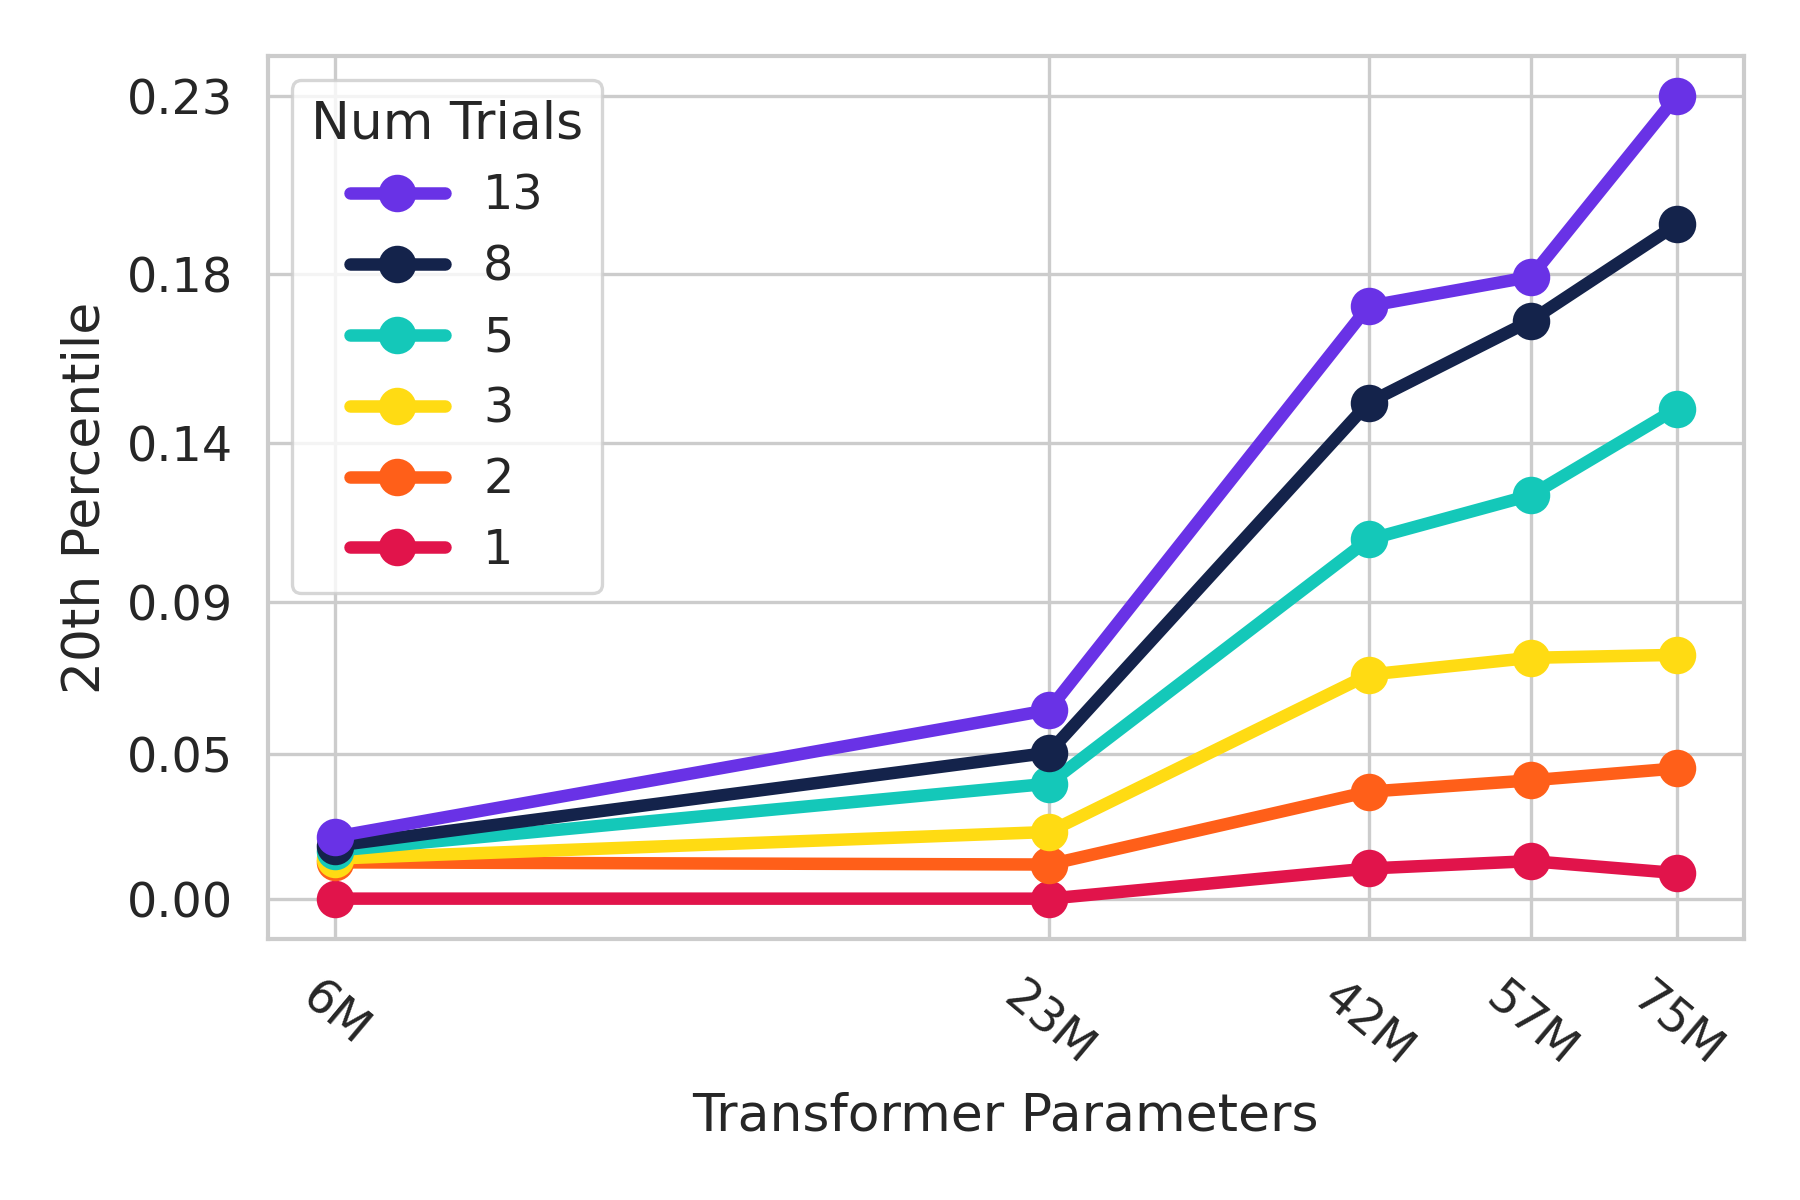
\includegraphics[width=\textwidth]{figures/scaling/worlds_complexity_parameter_scaling_percentile20.png}
        \caption{\centering Task distribution with many world topologies facilitates scaling (20th percentile).}
        \label{subfig:complexity-scaling-worlds-20th}
    \end{subfigure}
    \caption{The benefit of scaling model size is bottlenecked if the distribution is not complex enough, even if the total number of tasks is accounted for.}
\label{fig:task_complexity_scaling}
\end{figure}